\documentclass[tikz,border=3pt]{standalone}

\usepackage[T1]{fontenc}
\usepackage{libertine}
\usepackage{newtxmath}
\usepackage{xcolor}
\usetikzlibrary{arrows.meta,calc,positioning}

\renewcommand{\familydefault}{\sfdefault}

\definecolor{ink}{HTML}{20313F}
\definecolor{muted}{HTML}{667784}
\definecolor{line}{HTML}{A5B3BC}
\definecolor{panelbg}{HTML}{F8FAFB}
\definecolor{blue}{HTML}{2A6F97}
\definecolor{bluefill}{HTML}{EAF3F8}
\definecolor{teal}{HTML}{2A9D8F}
\definecolor{tealfill}{HTML}{E8F6F3}
\definecolor{orange}{HTML}{D97745}
\definecolor{orangefill}{HTML}{FFF1E8}

\tikzset{
  panel/.style={
    rounded corners=5pt,
    draw=line,
    line width=0.75pt,
    fill=panelbg,
    minimum height=5.40cm,
    align=center,
    text=ink,
    inner sep=0pt
  },
  stepbadge/.style={
    circle,
    minimum size=5.0mm,
    inner sep=0pt,
    text=white,
    font=\sffamily\bfseries\scriptsize
  },
  flow/.style={
    -{Latex[length=2.1mm,width=1.45mm]},
    draw=ink,
    line width=0.8pt,
    rounded corners=2pt
  },
  blueflow/.style={
    -{Latex[length=2.1mm,width=1.45mm]},
    draw=blue,
    line width=0.95pt,
    rounded corners=2pt
  },
  orangeflow/.style={
    -{Latex[length=2.1mm,width=1.45mm]},
    draw=orange,
    line width=0.95pt,
    rounded corners=2pt
  },
  chipblue/.style={
    rounded corners=3pt,
    draw=blue,
    fill=bluefill,
    line width=0.7pt,
    text=blue,
    inner xsep=4pt,
    inner ysep=2.5pt,
    font=\sffamily\scriptsize
  },
  chiporange/.style={
    rounded corners=3pt,
    draw=orange,
    fill=orangefill,
    line width=0.7pt,
    text=orange,
    inner xsep=4pt,
    inner ysep=2.5pt,
    font=\sffamily\scriptsize
  },
  statecaption/.style={
    fill=panelbg,
    rounded corners=1pt,
    inner xsep=0.8pt,
    inner ysep=0.8pt,
    font=\fontsize{6.2}{6.8}\selectfont,
    align=center
  },
  statecallout/.style={
    rounded corners=1.5pt,
    draw=blue!35,
    fill=panelbg,
    line width=0.35pt,
    inner xsep=1.0pt,
    inner ysep=1.0pt,
    font=\fontsize{6.0}{6.6}\selectfont,
    align=center,
    text=blue
  },
  statebox/.style={
    rounded corners=2pt,
    draw=blue,
    fill=white,
    line width=0.6pt,
    minimum width=10.5mm,
    minimum height=6.6mm,
    align=center,
    inner sep=1.5pt,
    text=ink
  }
}

\begin{document}
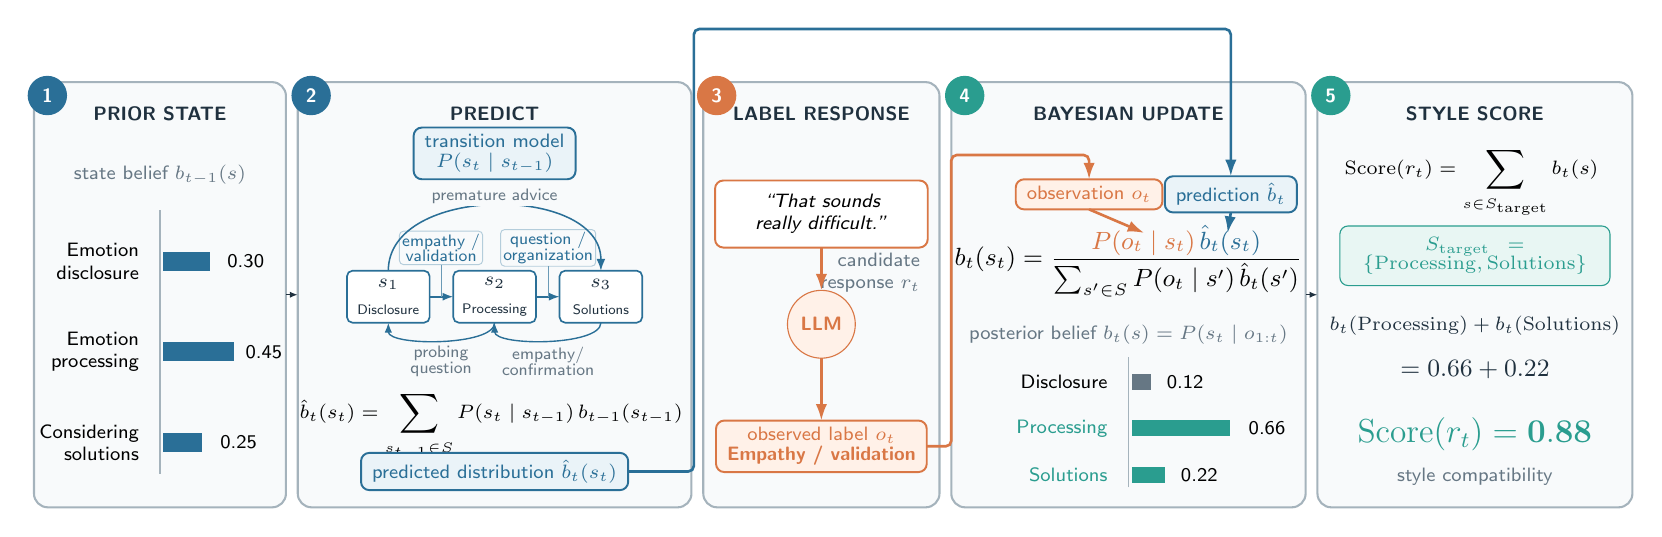
\begin{tikzpicture}[font=\sffamily, every node/.append style={outer sep=0pt}]
  % Five compact panels mirror the five operations described in the paper.
  \node[panel, minimum width=3.20cm] (prior) at (1.65,3.125) {};
  \node[panel, minimum width=5.00cm] (predict) at (5.90,3.125) {};
  \node[panel, minimum width=3.00cm] (observe) at (10.05,3.125) {};
  \node[panel, minimum width=4.50cm] (update) at (13.95,3.125) {};
  \node[panel, minimum width=4.00cm] (score) at (18.35,3.125) {};

  % Panel titles and numbered badges.
  \node[anchor=north, font=\sffamily\bfseries\scriptsize, text=ink]
    at ($(prior.north)+(0,-0.20)$) {PRIOR STATE};
  \node[anchor=north, font=\sffamily\bfseries\scriptsize, text=ink]
    at ($(predict.north)+(0,-0.20)$) {PREDICT};
  \node[anchor=north, font=\sffamily\bfseries\scriptsize, text=ink]
    at ($(observe.north)+(0,-0.20)$) {LABEL RESPONSE};
  \node[anchor=north, font=\sffamily\bfseries\scriptsize, text=ink]
    at ($(update.north)+(0,-0.20)$) {BAYESIAN UPDATE};
  \node[anchor=north, font=\sffamily\bfseries\scriptsize, text=ink]
    at ($(score.north)+(0,-0.20)$) {STYLE SCORE};

  \node[stepbadge, fill=blue] at ($(prior.north west)+(0.17,-0.17)$) {1};
  \node[stepbadge, fill=blue] at ($(predict.north west)+(0.17,-0.17)$) {2};
  \node[stepbadge, fill=orange] at ($(observe.north west)+(0.17,-0.17)$) {3};
  \node[stepbadge, fill=teal] at ($(update.north west)+(0.17,-0.17)$) {4};
  \node[stepbadge, fill=teal] at ($(score.north west)+(0.17,-0.17)$) {5};

  % Step 1: prior state distribution b_{t-1}.
  \node[font=\scriptsize, text=muted] at (1.65,4.65)
    {state belief \(b_{t-1}(s)\)};
  \draw[draw=line, line width=0.6pt] (1.65,0.85) -- (1.65,4.20);

  \node[anchor=east, align=right, font=\scriptsize] at (1.50,3.55)
    {Emotion\\disclosure};
  \fill[blue] (1.69,3.43) rectangle ++(0.60,0.24);
  \node[anchor=west, font=\scriptsize] at (2.39,3.55) {0.30};

  \node[anchor=east, align=right, font=\scriptsize] at (1.50,2.40)
    {Emotion\\processing};
  \fill[blue] (1.69,2.28) rectangle ++(0.90,0.24);
  \node[anchor=west, font=\scriptsize] at (2.62,2.40) {0.45};

  \node[anchor=east, align=right, font=\scriptsize] at (1.50,1.25)
    {Considering\\solutions};
  \fill[blue] (1.69,1.13) rectangle ++(0.50,0.24);
  \node[anchor=west, font=\scriptsize] at (2.30,1.25) {0.25};

  % Step 2: transition-model prediction.
  \node[chipblue, align=center] at (5.90,4.92)
    {transition model\\[-1pt]\(P(s_t\mid s_{t-1})\)};
  \node[statebox] (s1) at (4.55,3.10)
    {{\scriptsize \(s_1\)}\\[-2pt]{\tiny Disclosure}};
  \node[statebox] (s2) at (5.90,3.10)
    {{\scriptsize \(s_2\)}\\[-2pt]{\tiny Processing}};
  \node[statebox] (s3) at (7.25,3.10)
    {{\scriptsize \(s_3\)}\\[-2pt]{\tiny Solutions}};

  % The compact transition graph retains the strategies shown in state.pdf.
  \draw[-{Latex[length=1.35mm]}, draw=blue, line width=0.60pt]
    (s1.east) -- (s2.west);
  \draw[-{Latex[length=1.35mm]}, draw=blue, line width=0.60pt]
    (s2.east) -- (s3.west);
  \node[statecallout] (forwardone) at (5.22,3.72)
    {empathy /\\[-1pt]validation};
  \node[statecallout] (forwardtwo) at (6.58,3.72)
    {question /\\[-1pt]organization};
  \draw[draw=blue!70, line width=0.35pt]
    (forwardone.south) -- (5.22,3.10);
  \draw[draw=blue!70, line width=0.35pt]
    (forwardtwo.south) -- (6.58,3.10);

  \draw[-{Latex[length=1.25mm]}, draw=blue, line width=0.50pt]
    (s2.south)
    .. controls +(0,-0.30) and +(0,-0.30) ..
    (s1.south);
  \draw[-{Latex[length=1.25mm]}, draw=blue, line width=0.50pt]
    (s3.south)
    .. controls +(0,-0.30) and +(0,-0.30) ..
    (s2.south);
  \node[statecaption, text=muted] at (5.22,2.28)
    {probing\\[-1pt]question};
  \node[statecaption, text=muted] at (6.58,2.28)
    {empathy/\\[-1pt]confirmation};

  \draw[-{Latex[length=1.5mm]}, draw=blue, line width=0.55pt]
    (s1.north)
    .. controls +(0,1.10) and +(0,1.10) ..
    node[statecaption, text=muted, midway, above=0pt]
      {premature advice}
    (s3.north);

  \node[align=center, font=\scriptsize] at (5.90,1.45) {%
    \(\displaystyle
      \hat b_t(s_t)
      =\sum_{s_{t-1}\in S}
      P(s_t\mid s_{t-1})\,b_{t-1}(s_{t-1})
    \)
  };
  \node[chipblue] (predout) at (5.90,0.88)
    {predicted distribution \(\hat b_t(s_t)\)};

  % Step 3: candidate response is mapped to an observation label.
  \node[
    rounded corners=3pt,
    draw=orange,
    fill=white,
    line width=0.7pt,
    text width=2.42cm,
    align=center,
    inner xsep=4pt,
    inner ysep=5pt,
    font=\scriptsize
  ] (response) at (10.05,4.15)
    {\textit{``That sounds\\really difficult.''}};
  \node[
    anchor=east,
    align=right,
    font=\scriptsize,
    text=muted
  ] at (11.42,3.40) {candidate\\response \(r_t\)};
  \node[
    circle,
    draw=orange,
    fill=orangefill,
    minimum size=8.5mm,
    font=\sffamily\bfseries\scriptsize,
    text=orange
  ] (llm) at (10.05,2.75) {LLM};
  \draw[orangeflow] (response.south) -- (llm.north);
  \node[chiporange, align=center] (obsout) at (10.05,1.20)
    {observed label \(o_t\)\\[-1pt]\textbf{Empathy / validation}};
  \draw[orangeflow] (llm.south) -- (obsout.north);

  % Step 4: the two variables enter separate terms in the Bayesian update.
  \node[chiporange] (obsport) at (13.45,4.40)
    {observation \(o_t\)};
  \node[chipblue] (predport) at (15.25,4.40)
    {prediction \(\hat b_t\)};

  % A single typeset fraction keeps the numerator and denominator aligned;
  % the two numerator factors use standard mathematical juxtaposition.
  \node[font=\small] at (13.95,3.55) {%
    \(\displaystyle
      b_t(s_t)=
      \frac{
        {\color{orange}P(o_t\mid s_t)}
        \,{\color{blue}\hat b_t(s_t)}
      }{
        \sum_{s'\in S}P(o_t\mid s')\,\hat b_t(s')
      }
    \)
  };
  \draw[orangeflow] (obsport.south) -- (14.15,3.91);
  \draw[blueflow] (predport.south) -- (15.21,3.91);

  \node[font=\scriptsize, text=muted] at (13.95,2.62)
    {posterior belief \(b_t(s)=P(s_t\mid o_{1:t})\)};
  \draw[draw=line, line width=0.55pt] (13.95,0.68) -- (13.95,2.34);

  \node[anchor=east, font=\scriptsize] at (13.80,2.02) {Disclosure};
  \fill[muted] (13.99,1.92) rectangle ++(0.24,0.20);
  \node[anchor=west, font=\scriptsize] at (14.32,2.02) {0.12};

  \node[anchor=east, font=\scriptsize, text=teal] at (13.80,1.43) {Processing};
  \fill[teal] (13.99,1.33) rectangle ++(1.25,0.20);
  \node[anchor=west, font=\scriptsize] at (15.36,1.43) {0.66};

  \node[anchor=east, font=\scriptsize, text=teal] at (13.80,0.84) {Solutions};
  \fill[teal] (13.99,0.74) rectangle ++(0.42,0.20);
  \node[anchor=west, font=\scriptsize] at (14.50,0.84) {0.22};

  % Explicit input rails preserve the informative arrows from the source slide
  % while keeping them outside every text and equation block.
  \draw[blueflow]
    (predout.east)
    -- (8.43,0.88)
    -- (8.43,6.50)
    -- (15.25,6.50)
    -- (predport.north);
  \draw[orangeflow]
    (obsout.east)
    -- (11.70,1.20)
    -- (11.70,4.90)
    -- (13.45,4.90)
    -- (obsport.north);

  % Step 5: sum only the target-state posterior mass.
  \node[align=center, font=\scriptsize] at (18.35,4.55) {%
    \(\displaystyle
      \mathrm{Score}(r_t)=
      \sum_{s\in S_{\mathrm{target}}} b_t(s)
    \)
  };
  \node[
    rounded corners=3pt,
    draw=teal,
    fill=tealfill,
    text=teal,
    text width=3.15cm,
    align=center,
    inner xsep=4pt,
    inner ysep=4pt,
    font=\scriptsize
  ] at (18.35,3.62) {%
    \(S_{\mathrm{target}}=\)\\[-1pt]
    \(\{\mathrm{Processing},\mathrm{Solutions}\}\)
  };
  \node[font=\scriptsize, text=ink] at (18.35,2.73) {%
    \(b_t(\mathrm{Processing})+b_t(\mathrm{Solutions})\)
  };
  \node[font=\small, text=ink] at (18.35,2.18)
    {\(=0.66+0.22\)};
  \node[font=\bfseries\large, text=teal] at (18.35,1.35)
    {\(\mathrm{Score}(r_t)=\mathbf{0.88}\)};
  \node[font=\scriptsize, text=muted] at (18.35,0.82)
    {style compatibility};

  % Preserve the source figure's primary left-to-right flow with compact
  % connectors that remain entirely inside the gaps between adjacent panels.
  \draw[
    -{Latex[length=1.0mm,width=0.8mm]},
    draw=ink,
    line width=0.55pt
  ] (prior.east) -- (predict.west);
  \draw[
    -{Latex[length=1.0mm,width=0.8mm]},
    draw=ink,
    line width=0.55pt
  ] (update.east) -- (score.west);

\end{tikzpicture}
\end{document}
